\section[Wiring]{Wiring}

\subsection{Início do Wiring}
Barragán, um dos criadores do Wiring, define sua criação como "um ambiente de programação e uma placa de entrada / saída de prototipagem eletrônica para explorar as artes eletrônicas e a mídia tangível"\cite{Barragan2004}.

O projeto Wiring foi iniciado em 2003 durante o mestrado de Barragán pela Interaction Design Institute Ivrea (IDII), Italia \footnote{\url{http://wiki.wiring.co/wiki/About}}. Sua idéia era disponibilizar a designers e artistas uma plataforma eletrônica de fácil utilização, retirando a necessidade de estudo afundo em linguagens de programação e eletrônica fazendo o usuário ter maior foco no que de fato é sua expertise. Esta facilidade também poderia ser aplicada no ensino de programação e prototipagem nas escolas.

Barragán se formou com distinção, o único a conseguir tal fação na IDII em 2004.

No outono do mesmo ano, o Wiring foi utilizado em curso de inverno de computação física na IDII, sendo o nome do projeto Stranger Familiar, ministrado por nomes como Massimo Banzi, Heather Martin, Yaniv Steiner, Reto Wettach. Neste projeto foi proposto a criação de objetos domésticos incomuns porém interessantíssimos\footnote{\url{http://wiring.org.co/exhibition/images/book01.pdf}}

\subsection{Wiring e o Processing}

O Processing foi criado em 2001 por Ben Fry e Casey Reas. Seu objetivo era tornar a programação mais visual, facilitando a entrada de não-programadores ao meio da computação, principalmente voltado a artes e design.\cite{reas2007processing} A linguagem tem por base as capacidades gráficas da linguagem de programação Java. O Wiring foi desenvolvido através do Processing.

"Processing, como um subconjunto na linguagem Java, traz aos usuários uma interface de aplicativo independente da tecnologia na qual ele é usado, mantendo um nível de abstração que permite aos usuários aprender os fundamentos da programação de computadores e se concentrar em seus projetos ao invés de questões ou especificidades tecnológicas de uma plataforma. A linguagem de programação Java oferece uma sintaxe muito semelhante a C, C ++, Javascript ou Flash Actionscript, possibilitando a construção de programas e algoritmos que podem ser facilmente traduzidos para diferentes linguagens e ambientes. Isso faz do Processing uma ferramenta muito interessante para ensinar e aprender programação de computadores."\cite{Barragan2004}.

\subsection{Wiring e o Arduíno}

Ao contrário da relação entre Wiring e Processing, há uma grande discussão sobre o reconhecimento de o Arduíno ser uma derivação do Wiring.
Na página de créditos do Arduíno \footnote{\url{http://wiki.wiring.co/wiki/About}}, os autores informam que o Arduíno "(...)deriva do Wiring, uma plataforma construída por Hernando Barragán como sua tese de mestrado na Interaction-Ivrea" mas reforçam que o Wiring e, por sua vez, o Arduíno são derivados de um projeto chamado Massimo's Programma2003 (Figura \ref{programma2003}) e Processing, o último reconhecido por Barragán. 

\begin{figure}[htb]
	\caption{\label{programma2003}Placa Programma2003 projetada por Massimo Banzi em 2003}
	\begin{center}
	    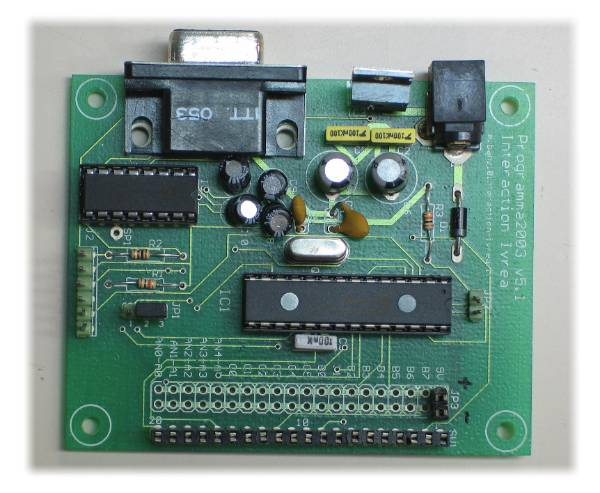
\includegraphics[scale=0.3]{refs/Programma2003}
	\end{center}
	%\legend{Fonte: Site da 3GPP}
\end{figure}

Já o criador do Wiring, criou uma página de nome "The Untold History of Arduino" \footnote{\url{https://arduinohistory.github.io/}} onde explica, em tom de crítica, diversos tópicos sobre o Arduíno.

%https://arduinohistory.github.io/
%http://wiki.wiring.co/wiki/About
%http://wiring.org.co/exhibition/images/book01.pdf
%https://www.arduino.cc/en/Main/Credits